\section{Policies}
   
   \subsection{Policies: Government Taxes to Exchanges}
   The first one is controlling the trading in the exchanges, this may be achieved through the government imposing taxes to the exchanges; as the exchanges have to pay to the government, they have to augment their own taxes (exchange fees), so this will represent a change in the price and obviously in the growth rate, as is shown in Figure \ref{img:polittaxes}.
   
   \begin{figure}[H]
      \centering
      \begin{subfigure}[t]{0.4\textwidth}
        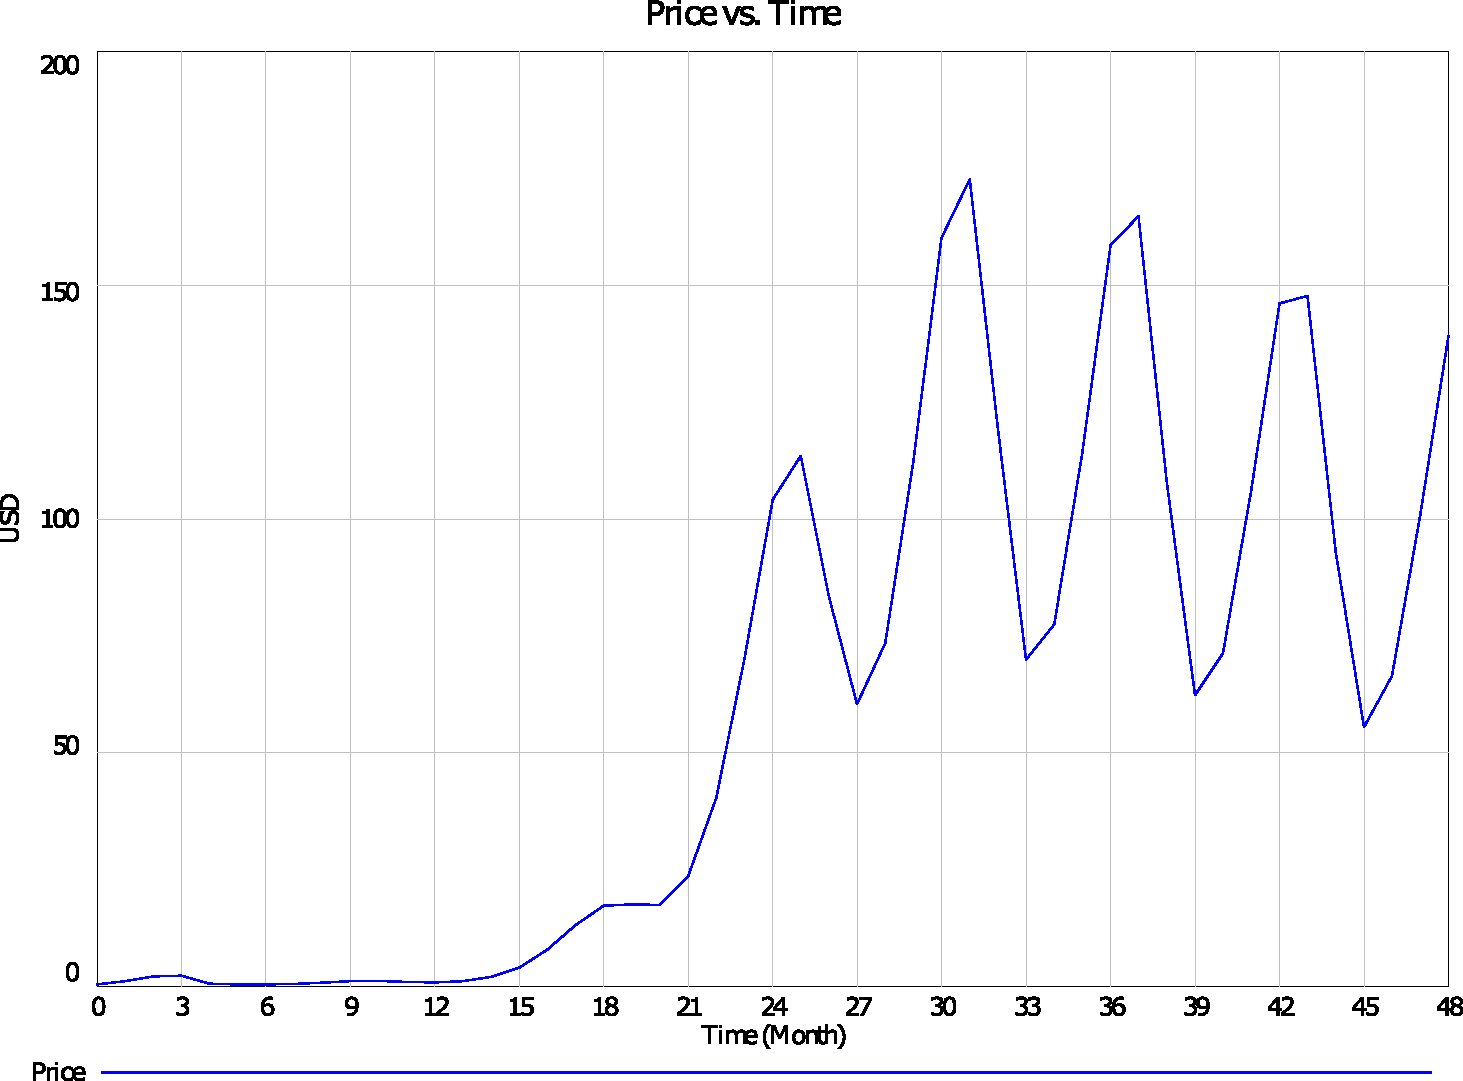
\includegraphics[scale = 0.3]{files/politTaxesPrice.pdf}
        \centering
        \caption{Results for price.}
      \end{subfigure}
      \hspace{1cm}
      \begin{subfigure}[t]{0.4\textwidth}
        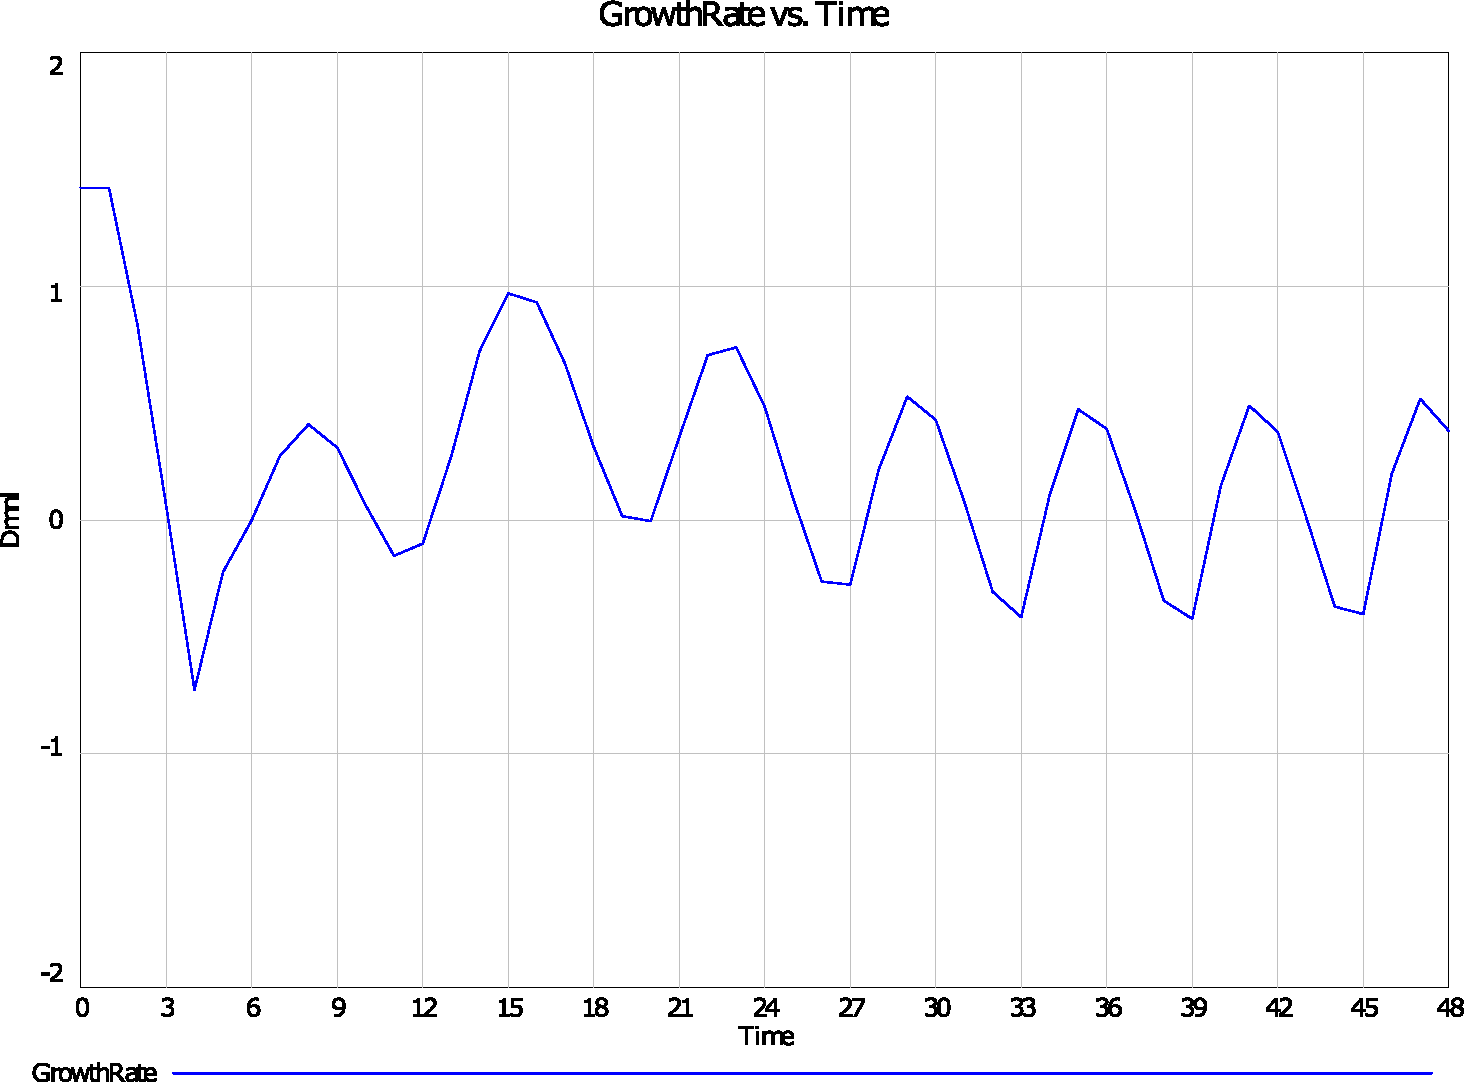
\includegraphics[scale = 0.3]{files/politTaxesGrowth.pdf}
        \centering
        \caption{Results for growth rate.}
      \end{subfigure}
      \caption{Results after setting government taxes.}
      \label{img:polittaxes}
	\end{figure}
   Note that the growth rate keeps a normal fluctuation and that the price is oscillating and tending to drop, as well as the price maximum is around 175USD, whereas the base model was around 480USD; this shows that the policy is effective and changes are taking place in the model results.
   
   
   \subsection{Policies: Limit the Number of New Investors}
   One of the most important factors that increase the price of a cryptocurrency is the number of investors that a certain cryptocurrency can handle. Therefore, it is of the utmost importance to regulate the number of investors that can enter the system monthly so the price grows in a more balanced way. The system was tested allowing only ten thousand people maximum to enter the system per month; in the real system, is not extremely hard to control this aspect but it needs government regulation to make it achievable. The results of this policy can be observed in Figure \ref{img:politinv}
   
    \begin{figure}[H]
      \centering
      \begin{subfigure}[t]{0.4\textwidth}
        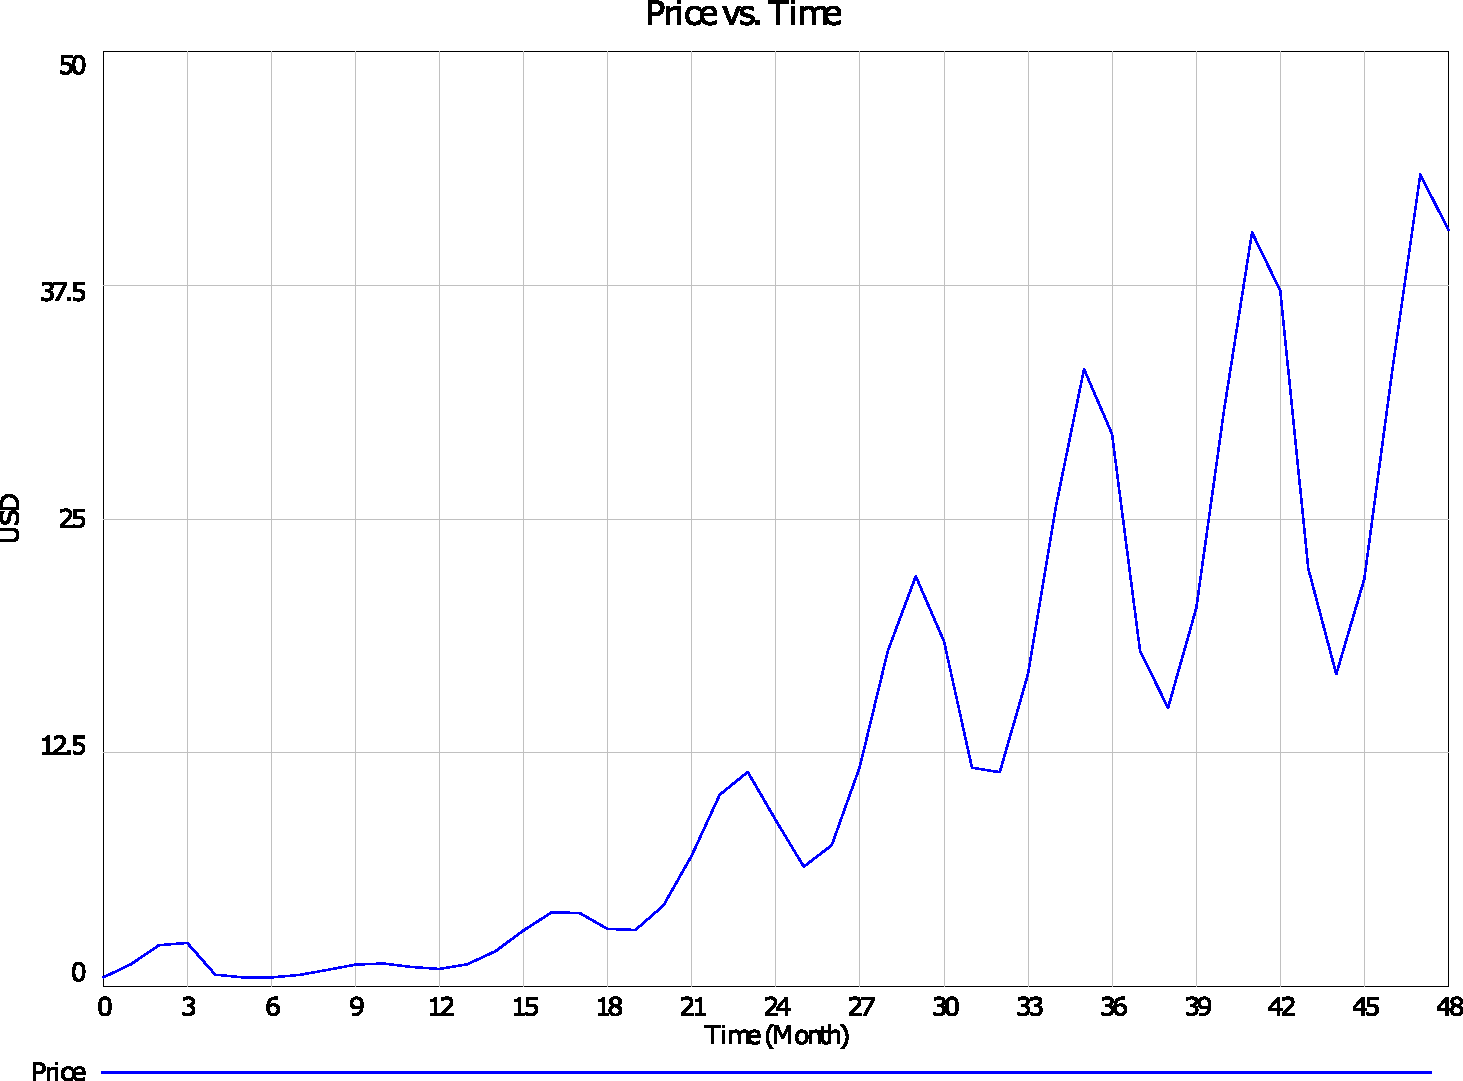
\includegraphics[scale = 0.3]{files/politInvPrice.pdf}
        \centering
        \caption{Results for price.}
      \end{subfigure}
      \hspace{1cm}
      \begin{subfigure}[t]{0.4\textwidth}
        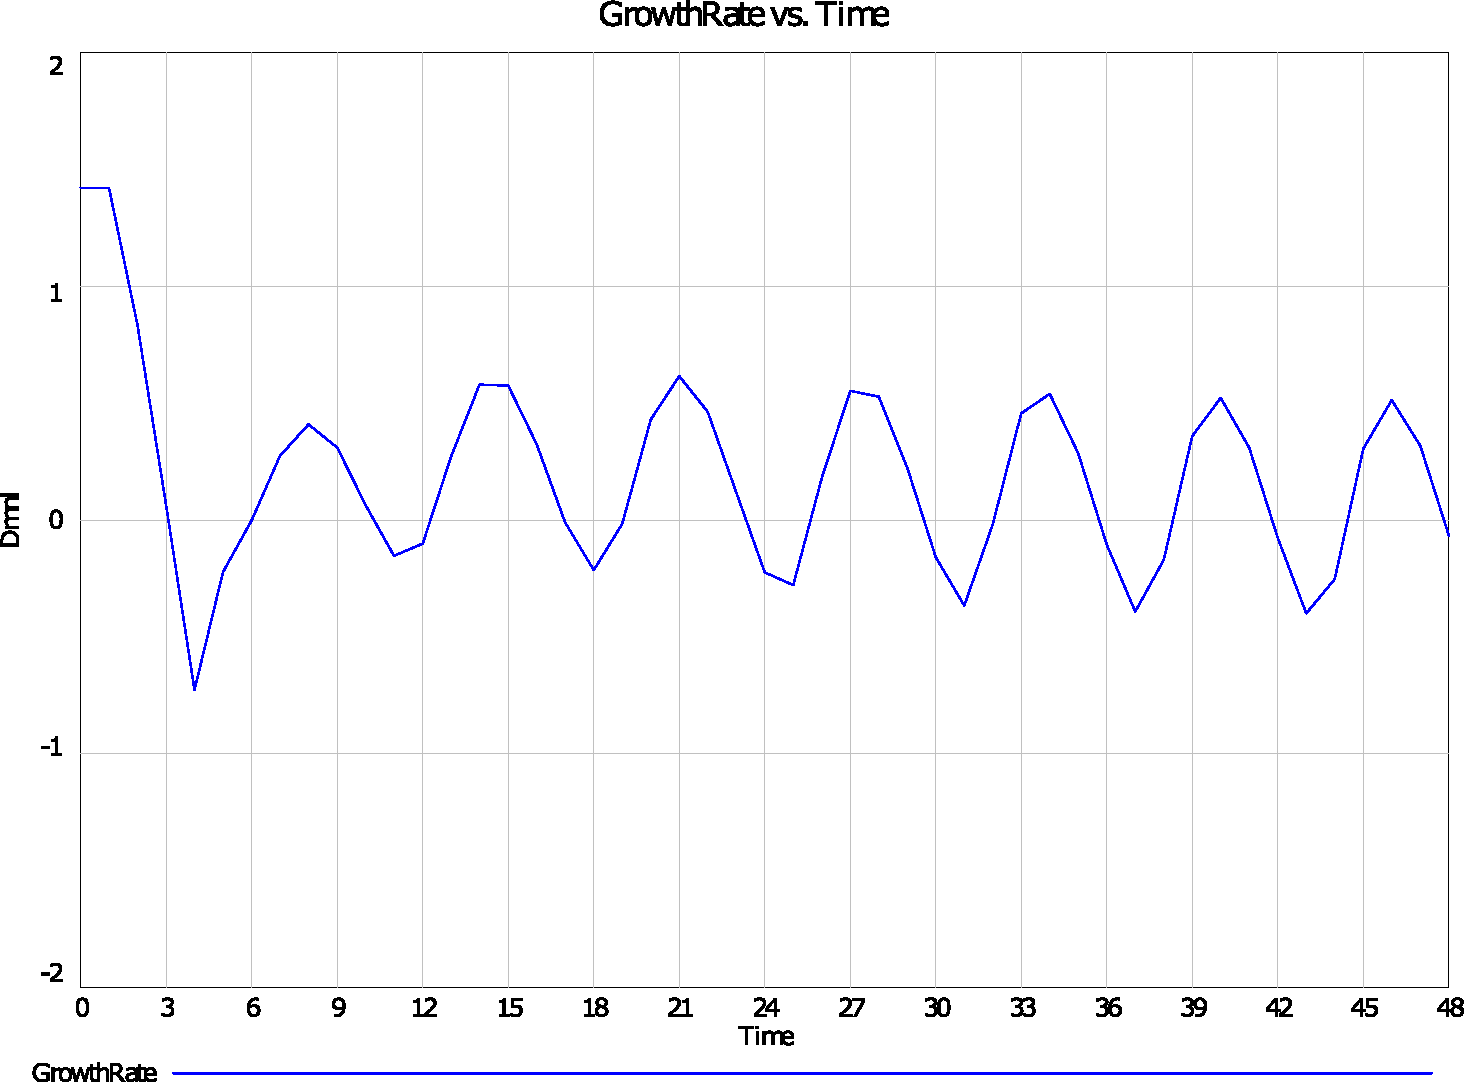
\includegraphics[scale = 0.3]{files/politInvGrowth.pdf}
        \centering
        \caption{Results for growth rate.}
      \end{subfigure}
      \caption{Results after limit in New Investors.}
      \label{img:politinv}
	\end{figure}
   
   \subsection{About policies}
   As it was previously presented, the policies can only be for external factors that affect the system; this is because the cryptocurrency system itself cannot be changed, as Silvio Micali \cite{silvio} states: ``A cryptocurrency cannot be fixed. If you ever want to change something, you would have to create a new one''. Therefore, we can only change external factors in order to make regulations without having to create a new currency.
